\chapter{Social Network User Interface}

In this chapter described the User Interface of Social Network implementated based on 104 mock-ups created by HCI expert team. The key design objective of the social network platform is to create a strong bond between (i) software engineering services for managing and deploying cloud-targeted application models; and (ii) community-oriented facilities for communication and
collaboration between users. The interconnections between the two in the design of the user interface are depicted in Figure \ref{fig:two_aspects}.
The prototype implementation is publicly accessible on-line at http://socialnetwork.paasage.eu. 

\begin{figure}[h]
	\caption{The engineering \& social activities are seamlessly within the Platform.}
	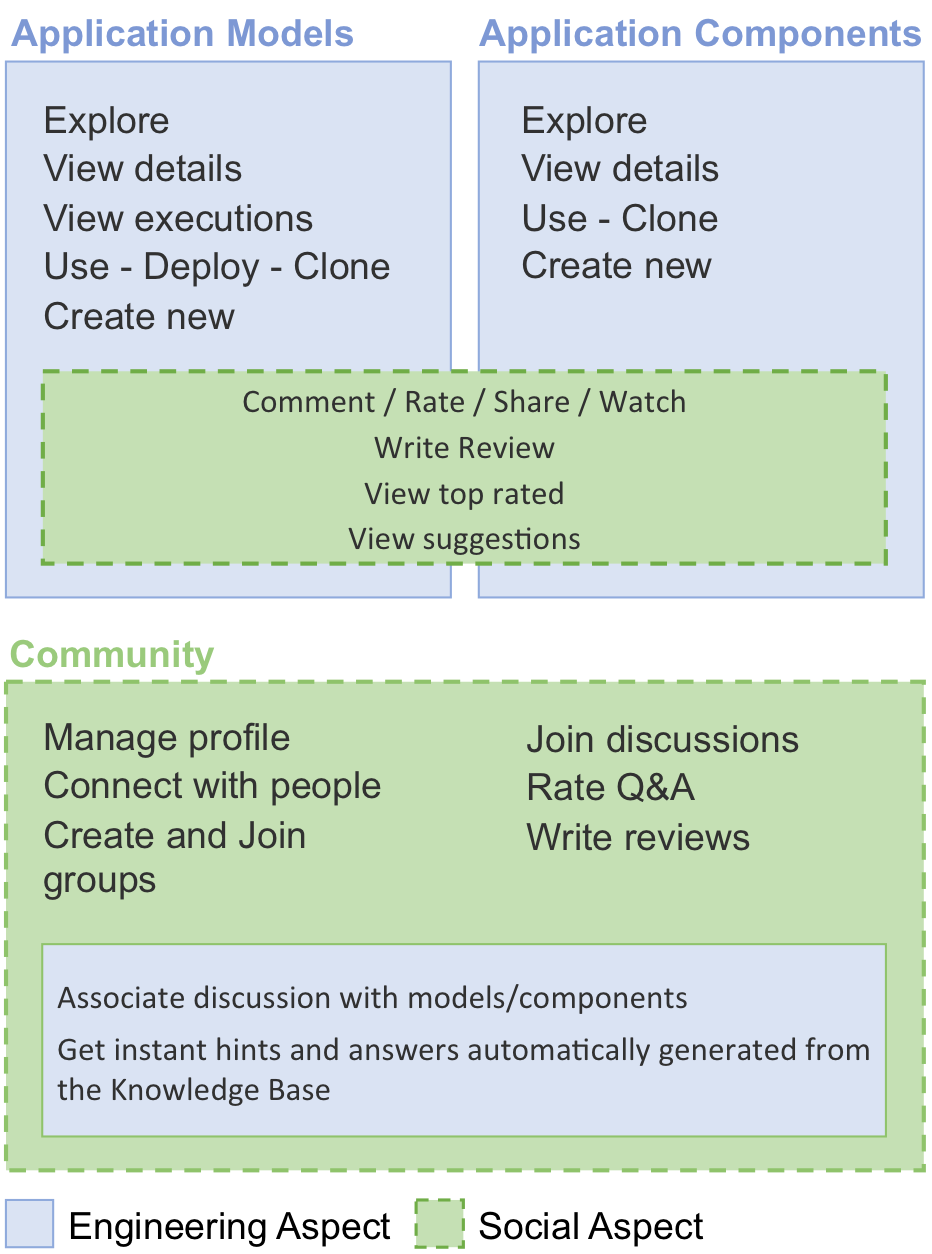
\includegraphics[width=0.6\textwidth,natwidth=200,natheight=150]{./fig/two_aspectes.png}
	\centering
	\label{fig:two_aspects}
\end{figure}

\section{User Interface}
The discrete entities, which bound together the Social Networking with model aspects of Platform are:
\begin{itemize}
\item \emph{Application Models}, An example is shown if figure \ref{fig:jenter_home}, consisting of a human friendly description (label 1 in fig.\ref{fig:jenter_home}), the Camel Description of the model (label 2 in fig.\ref{fig:jenter_home}), reviews about the model (label 3 in fig.\ref{fig:jenter_home}). An overview of engineering aspects such as version and runs (label 4 in fig.\ref{fig:jenter_home}) and an overview of social aspects such as share and watches (label 5 in fig.\ref{fig:jenter_home}) 
\item \emph{Components}
\item \emph{Groups}
\item \emph{Users}
\end{itemize}
\section{Gamification}

\begin{figure}[h]
	\caption{The application model home page}
	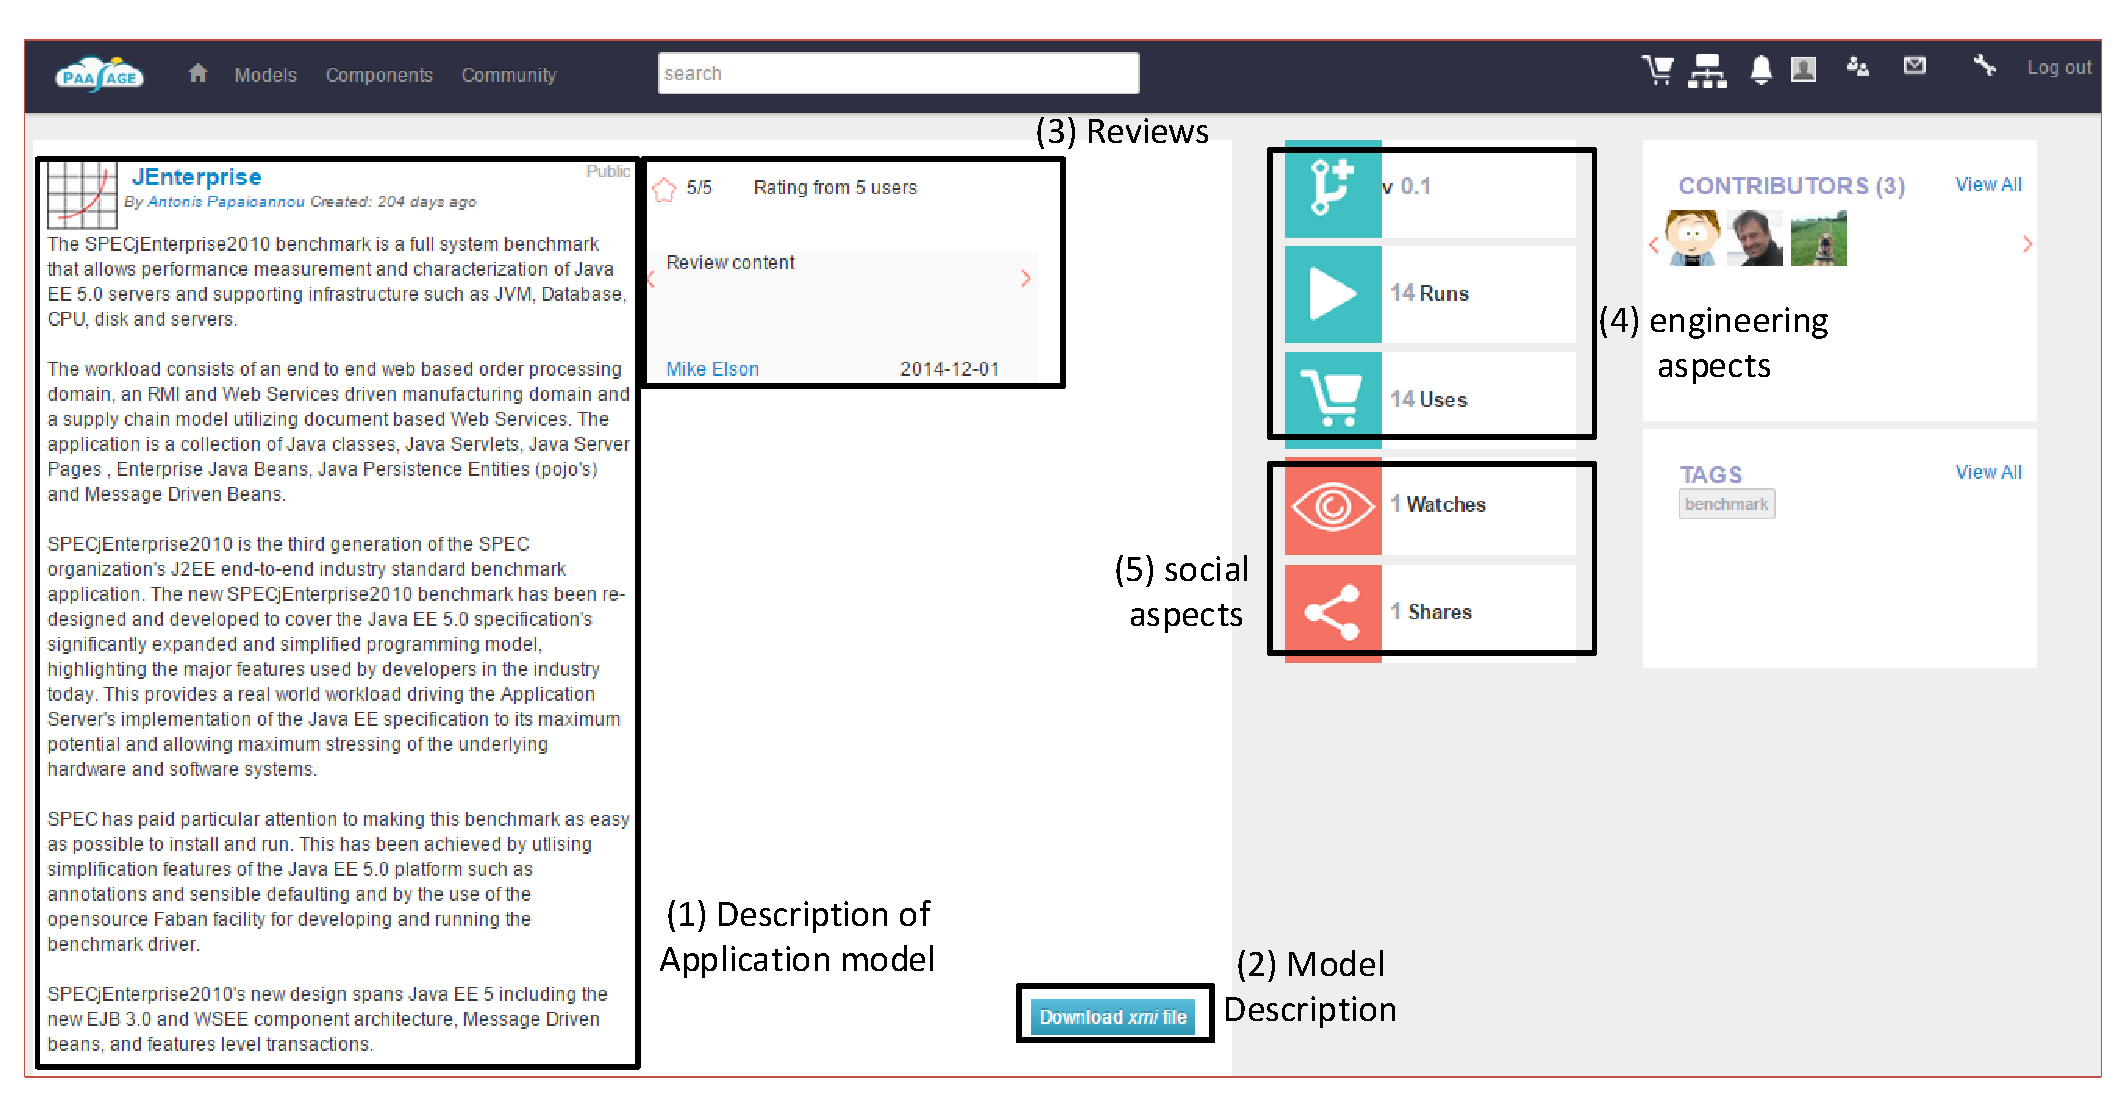
\includegraphics[width=1\textwidth,natwidth=200,natheight=150]{./fig/jenterprise_home_page.pdf}
	\centering
	\label{fig:jenter_home}
\end{figure}